% =============================================================================
% CS7980 Capstone paper — 6-PAGE CONFERENCE VERSION.
% Confirmatory campaign (E1 Qodo, E2 SWE-PRBench) + cross-family companion
% + E3 industrial arm + complexity interaction. All numbers replay from persisted
% artifacts with zero LLM calls (phase2-results/, hetero-confirmatory/,
% rap-portal-results/).
%
% TODO before submission:
%  1. OSF registration identifier/DOI + dates are still unfilled (Section III-C).
%  2. fig1_architectures_week11.png needs three edits so the image agrees with
%     the caption: (a) banner "ONLY THE COMMUNICATION TOPOLOGY CHANGES" ->
%     "EACH RUNG ADDS ONE CAPABILITY: SAMPLING -> SPECIALIZATION ->
%     COMMUNICATION"; (b) label the Hierarchical Coordinator and Synthesis boxes
%     "Deterministic" (they are code, not LLM calls -- that is why the arm shows
%     3 calls, not 5); (c) "Same Roles & Task Definitions" in the Held-Constant
%     row overclaims (Agentless and Generalists-3 have no roles).
%  3. Fig. 1's embedded title duplicates the LaTeX \caption (the page will show
%     the figure numbered twice). Crop it; also "Topologies" -> "Workflows".
%
% Reference check (2026-07-19): [11] pappu arXiv:2602.01011 and [13] zietsman
% arXiv:2603.25773 both verified against arXiv -- titles, author lists, and
% pappu's ICML 2026 acceptance all match. Bibliography is clean.
% =============================================================================

\documentclass[conference]{IEEEtran}
\IEEEoverridecommandlockouts

\usepackage{cite}
\usepackage{amsmath,amssymb,amsfonts}
\usepackage{graphicx}
\usepackage{booktabs}
\usepackage{textcomp}
\usepackage{xcolor}
\usepackage{url}

\begin{document}

\title{Evaluating Multi-Agent Review Workflows\\
for Automated Code Review: A Pre-Registered Study}

\author{\IEEEauthorblockN{En-Ping Su, Tong Wu, Shiting Huang, Mengshan Li}
\IEEEauthorblockA{\textit{Khoury College of Computer Sciences} \\
\textit{Northeastern University}, Vancouver, Canada}}

\maketitle

\begin{abstract}
Large Language Models are increasingly used for automated code review, and
multi-agent frameworks propose dividing the work among specialized agents. It
remains unclear whether the \emph{communication topology} among agents---rather
than their mere presence, or the extra compute they consume---improves review
quality. We compare a four-rung experimental \emph{ladder} that incrementally
introduces additional sampling, role specialization, and peer communication---an
Agentless single-LLM baseline, a compute-matched Generalists-3 control that
separates ``more compute'' from ``specialization,'' a Hierarchical
manager-plus-specialists design, and a Decentralized Peer Consensus
design---while holding the model, PR snapshot, prompt templates, and evaluation
pipeline fixed. Hypotheses and the analysis plan were pre-registered. We report
1{,}188 reviews over 99 injected-defect PRs, 600 over 50 human-reviewed PRs, and
627 over 30 PRs from a live industrial portal. Role specialization produced no
improvement over compute-matched generalist sampling ($p{=}0.73$), and Agentless
achieved the highest F1 among the tested arms (0.49 vs.\ 0.36--0.38, Holm
$p{<}0.001$); multi-agent workflows raised recall but required 3--9$\times$ the
per-run call budget. Separately, findings produced by three independent model
families matched injected ground truth 89\% of the time versus 54\% for findings
recurring across three runs of one model (reproduced under a second pair judge,
$\kappa{=}0.95$). On an unlabeled industrial repository this relationship could
not be validated: independent genuineness judges disagreed almost completely
($\kappa{=}0.03$). These results locate the clearest value of diversity in
cross-family verification rather than homogeneous multi-agent generation, while
showing that such verification requires a reliable correctness oracle.
\end{abstract}

\begin{IEEEkeywords}
Large Language Models, Multi-Agent Systems, Automated Code Review, Evaluation,
LLM-as-a-Judge.
\end{IEEEkeywords}

% =============================================================================
\section{Introduction}

Code review gates most software changes, and LLMs now plausibly automate parts
of it. A prominent design direction decomposes the task among specialized agents
that communicate, as in ChatDev~\cite{chatdev} and MetaGPT~\cite{metagpt}. Most
evaluations, however, compare a \emph{whole} multi-agent system against a single
model, conflating two variables: how many agents there are, and how they are
organized. A centralized manager may be cheaper; peer discussion may catch more
cross-component issues; or the structure may add cost without accuracy. We ask:

\begin{quote}
\textbf{RQ:} Holding the underlying model, review target, and evaluation
procedure fixed, what incremental effects do additional sampling, role
specialization, and inter-agent communication have on the effectiveness and
efficiency of automated code review?
\end{quote}

Answering this needs a control most studies omit. If a three-specialist team beats
a single reviewer, the cause may simply be three samples rather than three
\emph{roles}. We therefore add a compute-matched \textbf{Generalists-3} arm---the
same prompt sampled three times and merged---so specialization is tested against
equal compute, not against a single call. Agentless is a strong baseline, since
simple non-agent pipelines are competitive on software tasks~\cite{agentless}.

Because a benchmark result is only as trustworthy as its evaluation, we evaluate
on three complementary datasets---injected-defect ground truth, human-reviewer
agreement, and a live industrial repository---and pre-registered the hypotheses,
sample sizes, and analysis before collection. Our contributions are:
\begin{itemize}
  \item A pre-registered experimental ladder separating additional sampling,
  role specialization, and peer communication through adjacent contrasts, over
  2{,}415 reviews.
  \item Evidence that the tested homogeneous multi-agent workflows provide no F1
  improvement over the single-pass baseline, and that specialization adds nothing
  over compute-matched sampling.
  \item Identification of a \emph{cross-model verification} axis where
  multi-agent value does live---agreement between independent model families
  predicts golden-set matching far better than repeated sampling of one model.
  \item An external-validity boundary: on real unlabeled code that relationship
  could not be validated, because LLM correctness judges are mutually unreliable
  ($\kappa{=}0.03$)---a caution for LLM-judged evaluation generally.
\end{itemize}

% =============================================================================
\section{Related Work}

\textbf{LLM-based software engineering.} SWE-bench established that realistic
GitHub tasks are hard for language models~\cite{swebench}. Agentless questions
whether autonomous agent systems are necessary at all, showing a simple pipeline
is competitive~\cite{agentless}; it is the natural baseline for asking whether
multi-agent communication adds measurable value.

\textbf{Multi-agent software engineering.} ChatDev models development as
communication among role agents~\cite{chatdev}; MetaGPT adds structured workflows
to reduce inconsistency~\cite{metagpt}. Surveys find the area promising but
under-evaluated~\cite{survey}, and recent work catalogs \emph{why} multi-agent
LLM systems fail---coordination overhead, cascading errors, weak
verification~\cite{whyfail}. Concurrent 2026 results point the same way: agent
teams can hold individual experts back~\cite{pappu}, and mixing different models
does not beat the best single model on quality~\cite{selfmoa}. Our contribution
is a controlled experimental ladder that separates the effects of additional
sampling, role specialization, and peer communication through adjacent
contrasts, and shows where model diversity does pay.

\textbf{Verification and LLM judges.} LLM judges scale
evaluation~\cite{llmjudge}, verifier-based selection converts extra samples into
quality~\cite{cobbe}, and diverse judge panels can replace a single
judge~\cite{verga}; but judges show self-preference bias~\cite{panickssery} and
prompt-form sensitivity~\cite{sclar}. We use judges in two roles---an
\emph{objective} same-issue matcher and a \emph{subjective} genuineness
judge---and find the first reliable and the second not, which bounds LLM-judged
verification and gives a powered test of the correlated-error conjecture for AI
code review~\cite{zietsman}.

% =============================================================================
\section{Study Design}

\subsection{The four-rung ladder}
\label{sec:variables}
Each rung adds exactly one capability over its predecessor
(Fig.~\ref{fig:architectures}): (1)~\textbf{Agentless}---one LLM reviews the PR
in a single pass; (2)~\textbf{Generalists-3}---the same generalist prompt sampled
three times and merged, with no roles and no communication (the compute-matched
control that isolates sampling from specialization); (3)~\textbf{Hierarchical}---a
\emph{deterministic} coordinator routes the diff to frontend, backend, and
database specialists, whose findings a \emph{deterministic} synthesizer merges;
(4)~\textbf{Consensus}---the same specialists review independently, then exchange
findings and vote.

Coordination and aggregation in the Hierarchical arm are deterministic code, not
model calls, so its three LLM calls are exactly its three specialists; only
Consensus adds inference stages (nine calls). The model (Claude Haiku 4.5),
prompt templates, byte-identical per-PR snapshot, and evaluation pipeline are
fixed across arms, but sampling budget, roles, and message flow vary by
construction---that is what the ladder manipulates. Inference is therefore not
constant across all four arms, so we read \emph{adjacent} contrasts rather than
treating topology as a single isolated variable. Each (PR, arm) value is the mean
of three runs; run-to-run noise is small (mean within-PR SD of semantic F1
${\approx}0.01$ for the deterministic arms and ${\approx}0.05$ for the sampled
ones), and the headline ordering---Agentless top-F1 and the H2 recall tie---holds
in each of the three runs individually, so the conclusions are not an artifact of
averaging.

\begin{figure*}[t]
  \centering
  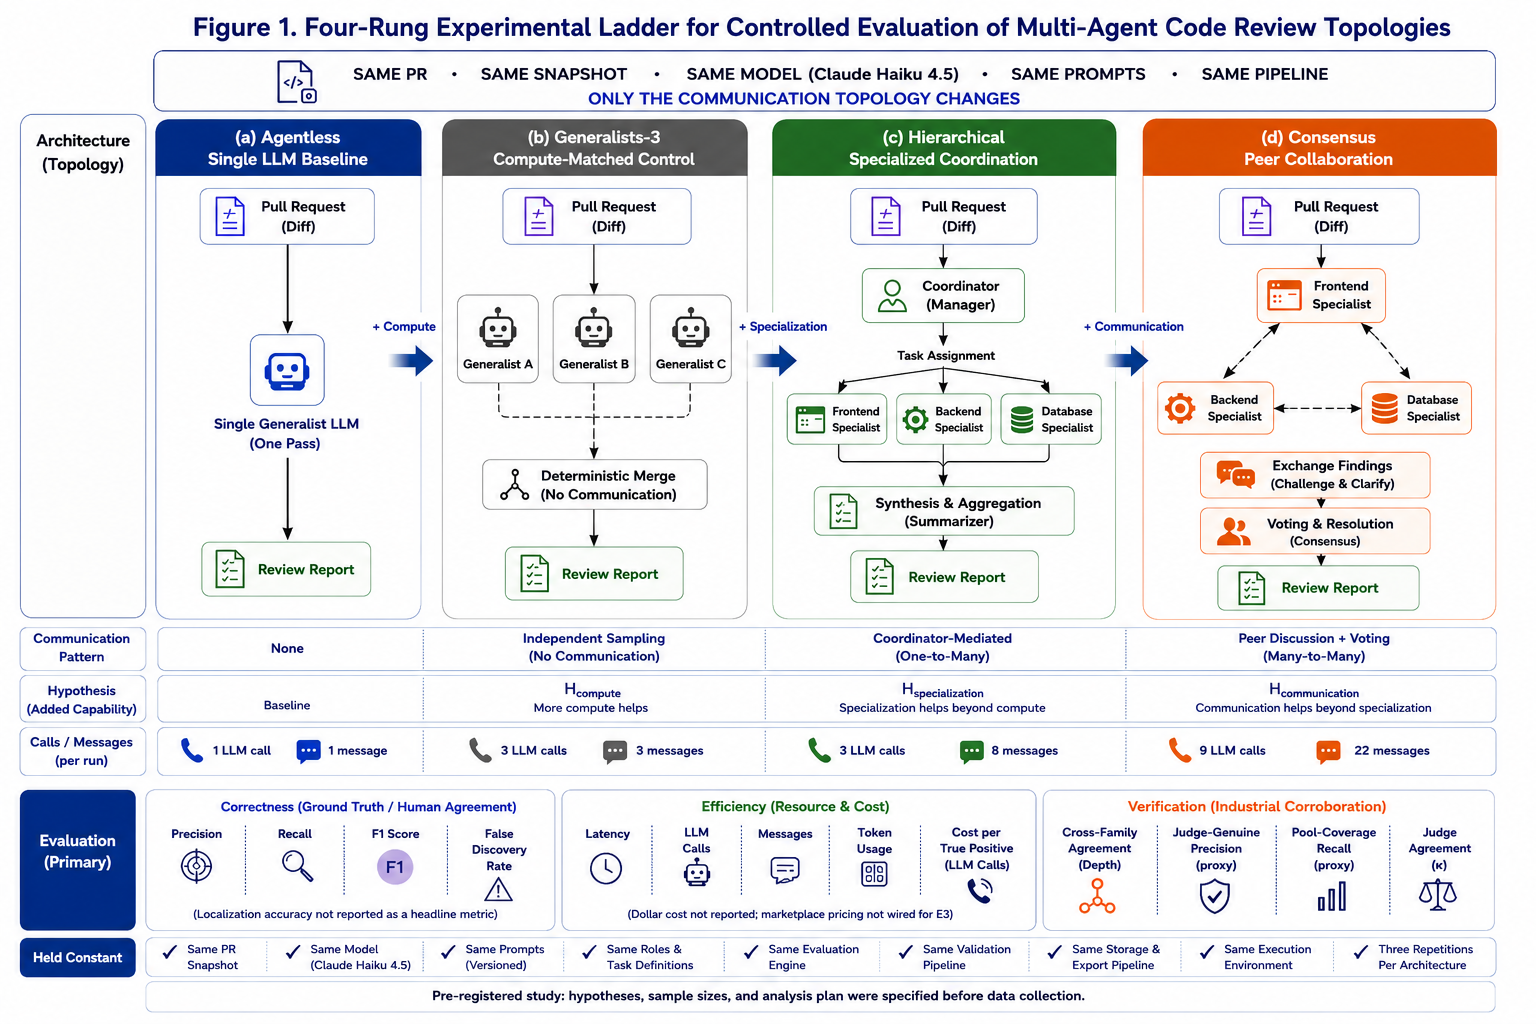
\includegraphics[width=\textwidth]{fig1_architectures_week11.png}
  \caption{The four-rung ladder. Each rung adds exactly one capability over its
  predecessor---sampling, then specialization, then communication---while the PR
  snapshot, model, prompt templates, and evaluation pipeline are held constant;
  inference budget necessarily varies with the rung, so we read \emph{adjacent}
  contrasts rather than treating topology as an isolated variable. Agentless
  reviews in a single pass; Generalists-3 samples the same generalist three times
  and merges deterministically without communication (the compute-matched
  control); Hierarchical routes through a \emph{deterministic} coordinator
  (one-to-many) and a \emph{deterministic} synthesizer, so its three LLM calls
  are exactly its three specialists; Consensus adds peer discussion and voting
  (many-to-many, nine calls). The per-run call and message counts beneath each
  rung are the coordination overhead quantified in
  Table~\ref{tab:confirmatory}.}
  \label{fig:architectures}
\end{figure*}

\subsection{Datasets and metrics}
\textbf{E1 --- Qodo PR-Review-Bench:} 99 PRs with injected defects and explicit
ground truth ($4\times3=1{,}188$ reviews), supporting objective
precision/recall/F1. \textbf{E2 --- SWE-PRBench:} 50 real PRs with human review
comments (600 reviews); metrics measure agreement with reviewers, not absolute
correctness. \textbf{E3 --- industrial:} 30 real merged PRs from an actively
developed full-stack portal, with no authoritative ground truth. Its 627 reviews
comprise the four-arm ladder ($4\times30\times3=360$) plus three single-pass
cross-family arms at three runs each: Haiku~4.5 (90), Kimi~K2.5 (90), and GLM~5
(87; GLM returned usable output on 29 of 30 PRs).

Findings are matched to ground truth both strictly (file$+$line) and
\emph{semantically}, where an independent LLM judge makes a binary same-issue
decision that rescues near-miss localizations; the judge is threshold-insensitive
across 0.5--0.9. Individual malformed findings are dropped and logged rather than
failing a whole review, removing a survivorship bias that previously penalized
the single-call arm. Operational metrics (latency, tokens, LLM calls, messages)
are collected identically everywhere.

For E3, which has no oracle, correctness is replaced by corroboration proxies
mirroring the E1 cross-family analysis. \emph{Corroboration depth} clusters
independent findings with an LLM pair judge (Nova Pro, $\tau{=}0.7$, union-find);
a cluster's depth is the number of independent model \emph{families} that
produced it. \emph{Proxy precision} is the per-arm rate at which a separate judge
rates findings genuine; \emph{proxy recall} is leave-one-out cross-family pool
coverage. The industrial axis is cross-\emph{family} (independent models), not
cross-architecture (one model, different topologies), because only the former
carries signal (Section~\ref{sec:hetero}).

\subsection{Hypotheses and analysis}
The design, hypotheses, sample sizes, and analysis plan were pre-registered on
OSF and prompts frozen before confirmatory collection. The registered contrasts
are summarized with their outcomes in Table~\ref{tab:hyp}. Two secondary
hypotheses were added by a pre-data amendment: \textbf{H-verify} (a
self-consistency filter lifts each multi-agent arm's F1 to within 0.02 of
Agentless) and \textbf{H-hetero-precision} (findings corroborated by ${\geq}2$ of
three independent families \{Haiku 4.5, Kimi K2.5, GLM~5\} gain ${\geq}10$
precision points at equal-or-higher F1, and all-three agreement exceeds the
frozen model's own three-run recurrence by ${\geq}10$ points).

The PR is the unit of analysis. Contrasts use paired Wilcoxon signed-rank tests
on per-PR differences, with seeded percentile-bootstrap CIs over those
differences and Holm--Bonferroni correction \emph{within} each hypothesis family
(families are not pooled). Cliff's $\delta$ is an unpaired dominance measure over
the two arms' per-PR distributions, so it complements rather than matches the
paired test: we read significance from Wilcoxon and magnitude from $\delta$. We
retain $\delta$ rather than a paired rank-biserial correlation because it answers
the deployment-relevant question directly---across PRs, how often does one arm
dominate the other---and because it is robust to the per-PR averaging over three
runs. \emph{Deviation:} the registration specified ``Cliff's $\delta$ (paired)'';
the implementation computes the standard unpaired dominance form. The registered
paired form (matched-pairs rank-biserial) nonetheless agrees on the primary
contrast---$r{=}{-}0.05$ versus the unpaired $\delta{=}{-}0.005$, both
negligible---so the choice is immaterial to the null. Since the
inferential claims rest on the paired Wilcoxon tests and their bootstrap CIs, and
$\delta$ is reported only as a magnitude, this does not affect any registered
conclusion, but we report the discrepancy rather than reconcile it silently. Every raw output and judge score is
persisted, so all statistics replay deterministically with zero new LLM calls.

% =============================================================================
\section{Results}
\label{sec:results}

\begin{table}[t]
\caption{Registered hypotheses and confirmatory outcomes.}
\label{tab:hyp}
\centering
\footnotesize
\begin{tabular}{@{}p{1.55cm}p{2.6cm}p{3.0cm}@{}}
\toprule
\textbf{Hypothesis} & \textbf{Prediction} & \textbf{Outcome} \\
\midrule
H-specialization \emph{(primary)} & Specialists beat compute-matched generalists & \textbf{Null} ($p{=}0.73$) \\
H-compute        & 3 samples beat 1 & Supported on recall (0.63 vs.\ 0.50), not F1 \\
H-communication  & Consensus beats Hierarchical & Unsupported (Holm $p{=}0.12$) \\
H-efficiency     & Cost rises along the ladder & Supported (monotonic) \\
H-complexity     & Effect grows with PR complexity & Registered test unavailable; not supported under an exploratory proxy \\
H-verify         & Self-consistency restores parity & \textbf{Fails} \\
H-hetero-prec.\  & Cross-family agreement lifts precision & \textbf{Confirmed} (both sub-claims) \\
\bottomrule
\end{tabular}
\end{table}

\subsection{Generation axis: more agents buy recall, never quality}
\label{sec:generation}
Table~\ref{tab:confirmatory} gives per-arm means over the 99 Qodo PRs together
with the cost of obtaining them. The \textbf{primary hypothesis is null}: at
matched compute, Hierarchical ties Generalists-3 on recall (0.624 vs.\ 0.626;
$p{=}0.73$, $\delta{=}{-}0.005$) at comparable precision. Beyond the
non-significant contrast, the recall difference is statistically
\emph{equivalent} within the pre-registered $\pm6$-point SESOI (two one-sided
tests, $p{<}0.001$; $90\%$ CI $[-0.025,0.019]$) and remains so at $\pm5$ points;
at $N{=}99$ the paired design detects $3.8$ recall points ($d_z{=}0.28$),
matching the registered power calculation, so the specialization effect is
bounded \emph{below} practical significance rather than merely undetected. Role
specialization
contributes nothing beyond sampling---consistent with concurrent evidence that
teams average rather than exploit expertise~\cite{pappu}. Nor does compute
convert into quality: Agentless dominates every multi-agent arm on semantic F1
(0.487 vs.\ 0.357--0.378; all Holm $p{<}0.001$, $\delta$ 0.30--0.36). What extra
compute buys is recall---Generalists-3 and Hierarchical reach 0.62--0.63 vs.\
0.503 (Holm $p{<}0.001$)---though Consensus, the most expensive arm, does not
(0.536, Holm $p{=}0.12$), leaving H-communication unsupported. Because Consensus
and Hierarchical differ in both communication pattern and inference budget
(nine calls vs.\ three), this contrast evaluates the complete peer-consensus
\emph{workflow} rather than communication in isolation: the tested workflow did
not outperform the hierarchical one despite its larger call and message budget.
The trade is stark (Fig.~\ref{fig:support}a): one confirmed finding costs 0.34
LLM calls under Agentless and 1.76 under Consensus, a $5\times$ premium for a
lower-F1 review. The operational ladder
rises monotonically in messages, latency, and cost-per-TP, confirming
H-efficiency.

On SWE-PRBench the shape replicates in natural data: Generalists-3 raises
coverage of human comments (0.68 vs.\ 0.51, Holm $p{=}0.001$; Hierarchical 0.63,
$p{=}0.05$), but F1 is a four-way tie (0.325 vs.\ 0.329--0.357, all n.s.,
$|\delta|{\le}0.06$). An exploratory Sonnet~4.5 pilot preserves the headline
claims---the single-pass F1 lead and the specialization null both hold---though
the Consensus arm's rank \emph{among} the multi-agent arms shifted; the
confirmatory robustness arm is deferred (Section~\ref{sec:threats}).

Finally, the pre-registered rescue fails. A self-consistency filter (keep
findings recurring in ${\geq}2$ of 3 runs) leaves Hierarchical at 0.378
($\tilde\Delta{=}{-}0.127$, CI $[-0.179,-0.083]$) and Consensus at 0.373
($\tilde\Delta{=}{-}0.114$), both entirely below the registered parity band;
$k{=}3$ fails for every arm. A model that agrees with itself is mostly repeating
its confident errors---which motivates the next section.

\begin{table}[t]
\caption{E1 (Qodo, 99 PRs): review quality and inference overhead. Agentless is
precision- and F1-dominant; extra agents buy recall at 3--9$\times$ the calls.
FDR $=1-$precision; Cost/TP $=$ LLM calls per confirmed true positive.}
\label{tab:confirmatory}
\centering
\footnotesize
\begin{tabular}{@{}lccccrrr@{}}
\toprule
\textbf{Arm} & \textbf{P} & \textbf{R} & \textbf{F1} & \textbf{FDR} & \textbf{Calls} & \textbf{Msgs} & \textbf{Cost/TP} \\
\midrule
Agentless      & \textbf{0.525} & 0.503 & \textbf{0.487} & \textbf{0.475} & 1 & 1  & \textbf{0.34} \\
Generalists-3  & 0.270 & \textbf{0.626} & 0.357 & 0.730 & 3 & 3  & 0.45 \\
Hierarchical   & 0.294 & 0.624 & 0.378 & 0.706 & 3 & 8  & 0.50 \\
Consensus      & 0.322 & 0.536 & 0.369 & 0.678 & 9 & 22 & 1.76 \\
\bottomrule
\end{tabular}
\end{table}

\subsection{Verification axis: cross-family agreement is a precision instrument}
\label{sec:hetero}
The registered companion generated agentless reviews with two independent
frontier families (Kimi K2.5, GLM~5, both clearing a pre-specified parity gate)
over the same PRs with the unchanged frozen prompt; cross-model
finding$\leftrightarrow$finding matching uses a fourth family (Nova Pro) as pair
judge, keeping the chain non-circular. The hypothesis was formed on a 20-PR pilot
subset, so it is tested on the registered 80-PR disjoint remainder of the
100-instance benchmark (the confirmatory ladder itself uses the 99 instances that
survived snapshot validation). There, \textbf{both sub-claims hold.} Findings corroborated by ${\geq}2$
families reach per-PR precision 0.716 vs.\ 0.575 single-arm
($\bar\Delta{=}{+}0.141$, CI $[0.094,0.189]$, $p{<}10^{-4}$, $\delta{=}0.364$) at
equal-or-higher F1. And findings all three families produce are golden-matched
\textbf{89\%} of the time versus \textbf{54\%} for findings the frozen model
repeats across all three of its own runs (gap ${+}0.348$, CI $[0.286,0.412]$).

Fig.~\ref{fig:depth} makes the mechanism visible. Cross-family agreement climbs
steeply with depth; same-model recurrence stays flat before saturating at its
error ceiling. A second run of the same model contributes almost no independent
evidence; a second independent family does. The instrument survives a change of
pair judge---re-judging all 8{,}061 candidate pairs with a second pair judge
agrees at $\kappa{=}0.952$ and reproduces the rows.

\begin{figure}[t]
\centering
% Generated by figures/make_figures.py (or figures/figures.ipynb). Regenerate
% with: cd figures && python3 make_figures.py
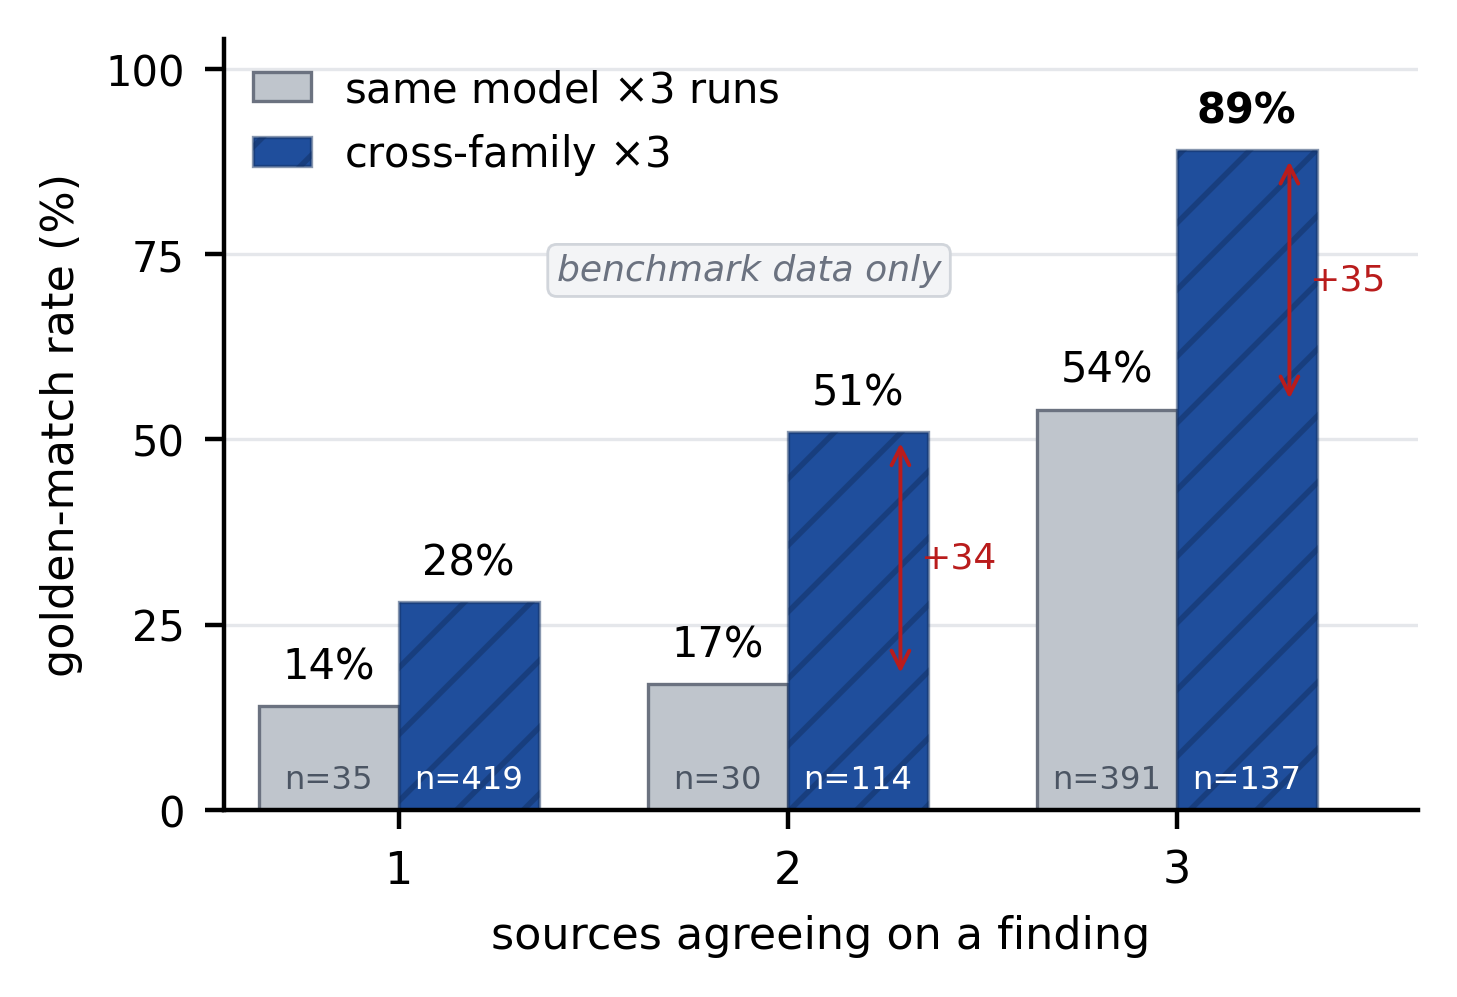
\includegraphics[width=\columnwidth]{fig2_depth_gradient.png}
\caption{Agreement predicts truth only when the agreeing sources are
\emph{independent}. Repeating one model three times barely improves on a single
run until full recurrence, and saturates at that model's error ceiling (54\%);
three independent families reach 89\%. The gap at equal depth---${+}34$ and
${+}35$ points---is the correlated-error mechanism made visible. This gradient
does not replicate on unlabeled industrial code (Section~\ref{sec:industrial}).}
\label{fig:depth}
\end{figure}

\subsection{Where the signal lives: functional bugs, not conventions}
\label{sec:signal}
Cross-family agreement is not uniformly informative---it concentrates on one
class of defect. Qodo injects two kinds, and stratifying the 80-PR set by them
separates them cleanly (Fig.~\ref{fig:support}b): universal \emph{functional} bugs
are recovered far more often at every depth than project-specific \emph{rule}
violations. The asymmetry has a simple cause. A null dereference or an unguarded
input is recognizable from the diff alone, whereas a repository-local convention
is invisible to a generic reviewer that has never seen the project's standards.
Independent families converge precisely where the defect is universal.

This shapes what the trust signal is \emph{for}. The ${\geq}2$-family set is 52\%
functional true positives, 20\% rule true positives, and 28\% golden-unmatched,
so cross-family agreement belongs as a high-precision filter for correctness
defects---not as a substitute for project-specific linting, which needs
repository context rather than more reviewers.

\begin{figure*}[t]
\centering
% Generated by figures/make_figures.py (or figures/figures.ipynb).
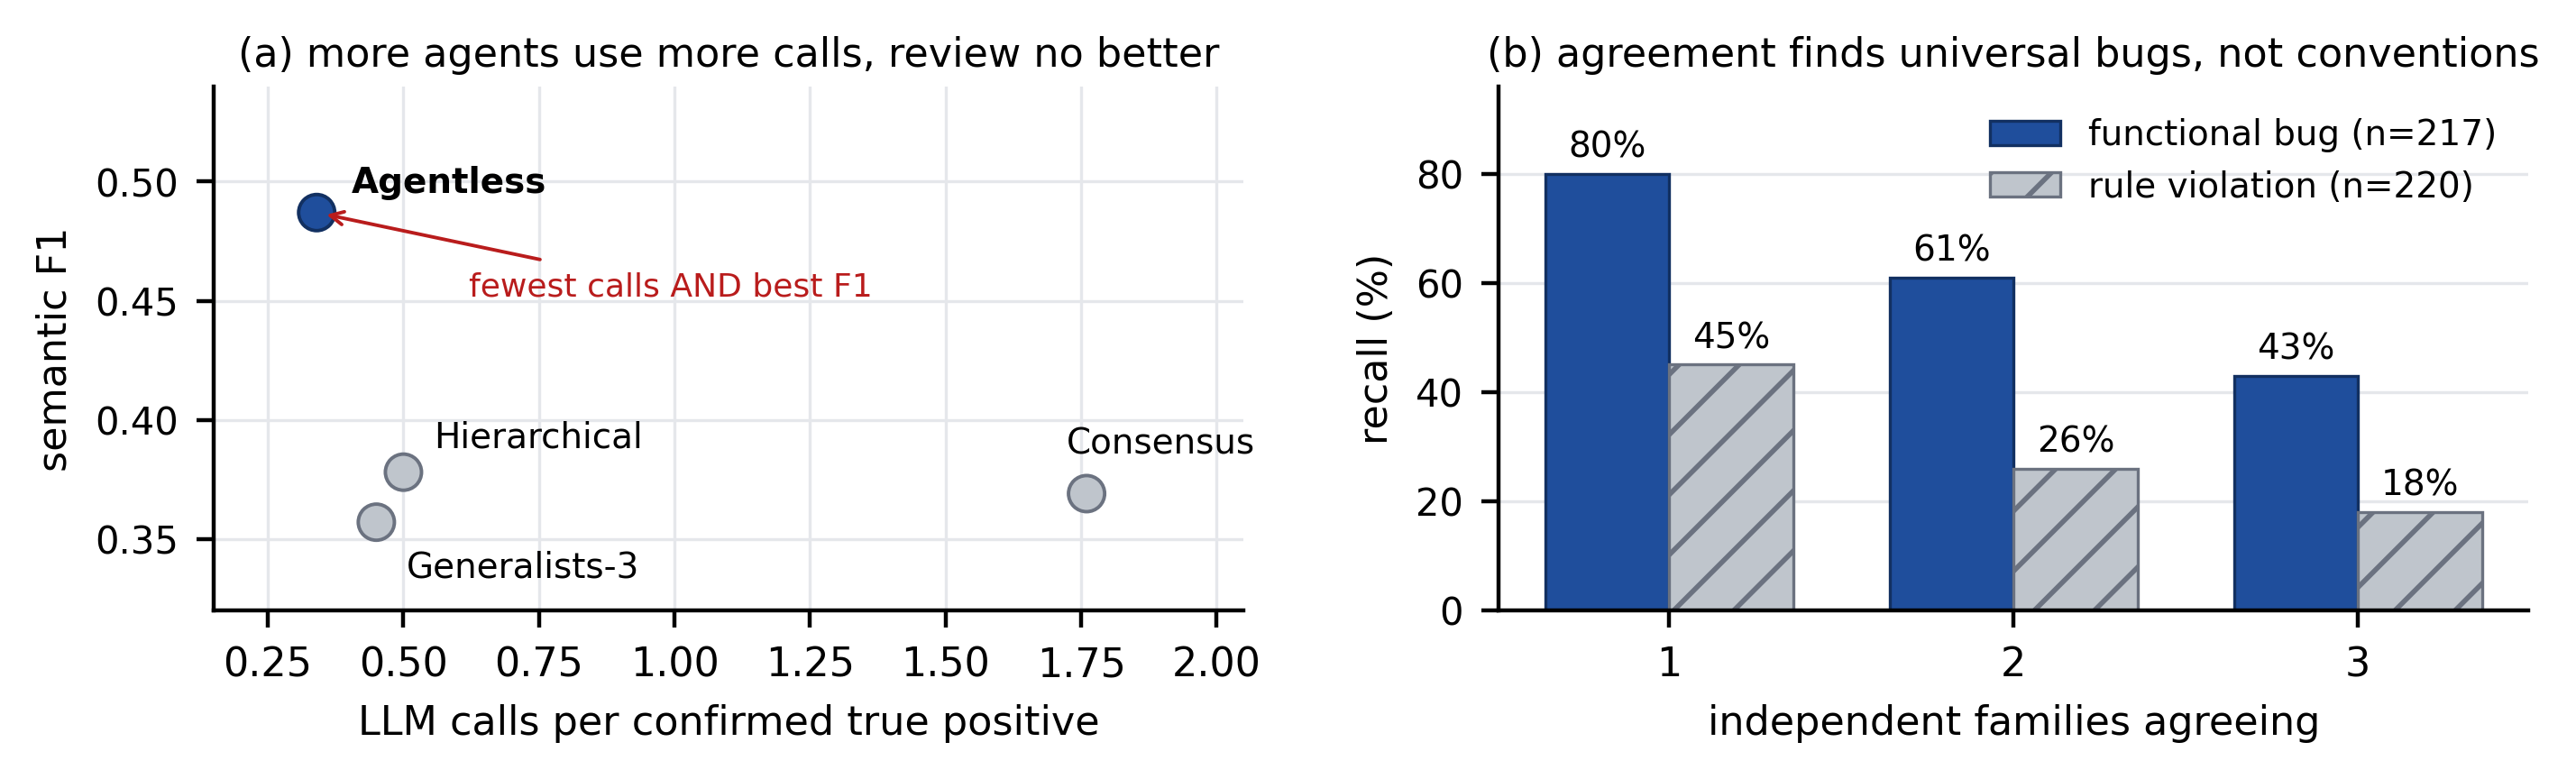
\includegraphics[width=\textwidth]{fig3_support.png}
\caption{Two supporting views of the same conclusion. \textbf{(a)} The
accuracy/cost frontier: Agentless Pareto-dominates---it is simultaneously the
cheapest arm (0.34 LLM calls per confirmed true positive) and the most accurate
(semantic F1 0.487), while Consensus costs $5\times$ more for a worse review.
\textbf{(b)} Where cross-family agreement carries signal: universal functional
bugs are recovered far more often at every depth than project-specific rule
violations, which a reviewer without repository context cannot know. Together,
the panels show that homogeneous multi-agent workflows increase inference cost
without improving F1, while cross-family corroboration is most informative for
universal functional defects.}
\label{fig:support}
\end{figure*}

\subsection{How complete is the oracle?}
\label{sec:completeness}
Every precision figure above is measured against the injected golden set, so its
completeness bounds their interpretation. We audited it confirmatorily: three
independent judge families read every golden-\emph{unmatched} finding against the
diff (``does this identify a genuine problem?''), plus a calibration pass on
golden-\emph{matched} findings. Llama~3.3 calls 76\% of unmatched findings real
(92\% on known defects); Mistral Large~3 calls 73\% (90\%); DeepSeek~V3.2 calls
only 33\% (71\%).

The disagreement is definitional, not a capability gap: DeepSeek is a strict
under-caller that rejects roughly 29\% of \emph{known injected defects}---largely
rule and style violations---while the lenient judges accept warranted concerns.
Critically, inter-judge agreement here is poor ($\kappa{=}0.23$--$0.58$) against
the pair judge's $\kappa{=}0.95$ on same-issue matching. This gap is not a
base-rate artifact of $\kappa$: under the prevalence-robust Gwet's AC1 and PABAK
the disagreement between the strict judge and the two lenient ones is if
anything sharper (AC1 $0.11$--$0.21$), while the two lenient judges agree
substantially (raw $84\%$, AC1 $0.74$); the same-issue matcher, by contrast,
stays high under every coefficient (AC1 $0.96$, PABAK $0.96$). Two questions that look
alike behave differently: whether two findings describe the same issue is
objective and stable across judges; whether a finding is a real bug is not settled by
an LLM judge of any size.

Three conclusions survive every definition. The golden set is materially
incomplete, so golden-referenced precision \emph{understates} all arms equally,
leaving relative comparisons intact. The ${\geq}2$-family set's effective
precision is bracketed at 86--95\%. And false positives are less false than they
appear: 21--32\% are localization near-misses---real defects at the wrong
line---and high-severity findings are almost always real. The magnitude awaits
human adjudication; the direction does not. The audit also predicts what follows:
remove the golden set, as the industrial arm does, and the only correctness
signal left is the one that was already unreliable.

\subsection{Industrial validation: the instrument needs an oracle}
\label{sec:industrial}
We ran the registered industrial arm on 30 real merged PRs (627 reviews: the
four-arm ladder plus the cross-family axis), scored with the same instruments but
with proxies in place of golden labels. Two patterns transfer. The
communication-cost ladder is unchanged (Agentless 1 call / 13\,s through
Consensus 9 calls / 173\,s), and the pool-coverage proxy gives the same
qualitative verdict---more agents do not buy coverage: the single-pass baseline
is highest (0.27) and the most-agentful Consensus lowest (0.10). (Pool coverage
is a different construct from golden recall---on which Agentless ranked
\emph{lowest}---so we compare directions, not ranks.)

The verification instrument, however, could not be \emph{validated} on unlabeled
code---the gradient of Fig.~\ref{fig:depth} cannot be measured here. Cross-family
agreement is rare: only 23
findings reach depth-2 and 5 reach depth-3 of 904 clusters, versus 114 and 137 on
E1. More decisively, the genuineness judges disagree almost completely---Nova
rates 99\% of findings genuine (a rubber stamp), DeepSeek 68\%, at
$\kappa{=}0.03$---so the depth$\rightarrow$precision relation is set by judge
choice, not corroboration: flat at 100\% under Nova, and \emph{inverted} under
the discriminating judge, where findings families agree on score 0\% versus 15\%
for solo findings. This is precisely the failure
Section~\ref{sec:completeness} anticipated, now with no golden set left to bound
it: the objective matcher still works, and the correctness judge does not. The
negative result is therefore about the \emph{measurement apparatus}, not the
underlying signal---with mutually inconsistent oracles and depth counts of 23 and
5, cross-family agreement can here be neither confirmed nor refuted.

\subsection{Complexity interaction: the effect does not grow with PR complexity}
\label{sec:rq3}
The registered stratifier was PR type, which requires the diff; the confirmatory
runs did not persist it, so we substitute the closest available proxy---the
number of distinct files an instance's defects span---and label this analysis
\textbf{exploratory}. \textbf{No interaction survives on any contrast} (all Holm
$p{\ge}0.42$, $|\delta|{\le}0.12$, Spearman $|\rho|{\le}0.17$). Complexity
degrades every arm by a similar margin (recall 0.52$\to$0.46 Agentless,
0.65$\to$0.56 Generalists-3 and Hierarchical, 0.57$\to$0.45 Consensus) and the
ordering is stable, so no topology rescues complex PRs. The one directional hint
runs \emph{against} the registered prediction: Consensus minus Hierarchical
recall is 0.000 on simple PRs and $-0.119$ on complex ones (Holm $p{=}1.0$)---a
non-significant counter-directional trend, not a finding.

% =============================================================================
\section{Threats to Validity}
\label{sec:threats}

\textbf{Construct.} E3 has no ground truth, so its metrics are proxies and are
labelled as such. Even the benchmark's golden set is incomplete
(Section~\ref{sec:completeness}), so golden-referenced precision is a lower bound;
relative comparisons are unaffected, because incompleteness applies to every arm
identically. The pair judge is validated instrument-side ($\kappa{=}0.95$) but its
human validation is pending, so corroboration numbers remain instrument-relative.

\textbf{Internal.} Differences could stem from confounds other than the
manipulated capability. We hold the model, prompt templates, evaluation pipeline,
and a byte-identical PR snapshot fixed while manipulating sampling budget, role
structure, and communication according to the experimental ladder; the
compute-matched Generalists-3 control separates specialization from raw sampling,
and the evaluation engine replays deterministically from stored artifacts.

\textbf{External.} Qodo is a synthetic-injection benchmark: planted defects are
cleaner and more localizable than natural review targets, so absolute scores sit
on a favorable setting even though within-benchmark comparisons hold; the
SWE-PRBench replication and the industrial arm partly offset this. One registered
piece is deferred---the Sonnet~4.5 robustness arm at confirmatory scale, whose
cost is prohibitive at $99\times4\times3$---so the exploratory pilot stands in its
place and single-model-family generalizability, specifically the ranking
\emph{within} the multi-agent arms, is stated as a limitation rather than claimed.
The industrial repository is partly AI-authored, which is disclosed.

\textbf{Conclusion.} The headline claims (the specialization null, Agentless F1
dominance, H-verify's failure, and both H-hetero sub-claims) are confirmatory:
registered sample sizes, paired tests, effect sizes with CIs, and Holm correction
within families. The finer stratifications and RQ3 are exploratory and labeled as
such; E3's depth-2/3 counts are small (23 and 5), so those CIs are wide.

% =============================================================================
\section{Conclusion}

Under a pre-registered, frozen-model design, none of the tested multi-agent
workflows improved automated code review. Role specialization adds nothing over
compute-matched sampling (the primary null), no arm exceeds the single-pass
baseline's F1, extra agents buy recall at a 3--9$\times$ larger per-run call
budget, the self-consistency rescue our own pilot suggested does not replicate,
and the effect does not grow with PR complexity. The \emph{verification} axis is
where multi-agent value lives: agreement between independent model families is a
registered precision instrument that survives a change of pair
judge---findings all three families produce match injected ground truth 89\% of
the time versus 54\% for one model repeating itself---and the signal concentrates
on functional bugs.

That instrument, however, has a precondition. On real unlabeled code we could not
validate it, because LLM correctness judges disagree at $\kappa{=}0.03$ while the
objective same-issue matcher stays reliable at $\kappa{=}0.95$; the industrial
result therefore bounds \emph{oracle-based validation}, not cross-family
agreement itself, which remains untested outside the labeled setting. The
practical guidance follows that boundary: on review tasks resembling the
benchmarked ones, do not add homogeneous agents for quality, and treat
cross-family agreement as a candidate trust signal to be calibrated against a
project's own oracle before it is relied upon. Future work is a fixed-definition
\emph{human} adjudication, the one oracle these judges could not provide.

\section*{Acknowledgment}
The authors thank their capstone advisors Lino Coria Mendoza and Yvonne Coady for
their guidance, and the Indigenomics Institute for access to the industrial
case-study repository.

\begin{thebibliography}{16}

\bibitem{chatdev}
C.~Qian et al., ``ChatDev: Communicative agents for software development,''
in \emph{Proc. ACL}, 2024.

\bibitem{metagpt}
S.~Hong et al., ``MetaGPT: Meta programming for a multi-agent collaborative
framework,'' in \emph{Proc. ICLR}, 2024.

\bibitem{agentless}
C.~S. Xia, Y.~Deng, S.~Dunn, and L.~Zhang, ``Agentless: Demystifying
LLM-based software engineering agents,'' arXiv:2407.01489, 2024.

\bibitem{swebench}
C.~E. Jimenez et al., ``SWE-bench: Can language models resolve real-world
GitHub issues?'' in \emph{Proc. ICLR}, 2024.

\bibitem{survey}
X.~Zhang et al., ``LLM-based multi-agent systems for software engineering:
Literature review, vision and the road ahead,'' arXiv preprint, 2024.

\bibitem{whyfail}
Y.~Li et al., ``Why do multi-agent LLM systems fail?'' arXiv preprint, 2025.

\bibitem{llmjudge}
L.~Zheng et al., ``Judging LLM-as-a-judge with MT-Bench and Chatbot Arena,''
in \emph{Proc. NeurIPS}, 2023.

% --- new references (week-12); author lists verified against arXiv. ---
\bibitem{cobbe}
K.~Cobbe, V.~Kosaraju, M.~Bavarian, M.~Chen, H.~Jun, L.~Kaiser, M.~Plappert,
J.~Tworek, J.~Hilton, R.~Nakano, C.~Hesse, and J.~Schulman, ``Training
verifiers to solve math word problems,'' arXiv:2110.14168, 2021.

\bibitem{verga}
P.~Verga, S.~Hofst\"atter, S.~Althammer, Y.~Su, A.~Piktus, A.~Arkhangorodsky,
M.~Xu, N.~White, and P.~Lewis, ``Replacing judges with juries: Evaluating LLM
generations with a panel of diverse models,'' arXiv:2404.18796, 2024.

\bibitem{panickssery}
A.~Panickssery, S.~R. Bowman, and S.~Feng, ``LLM evaluators recognize and
favor their own generations,'' arXiv:2404.13076, 2024.

\bibitem{pappu}
A.~Pappu, B.~El, H.~Cao, C.~di~Nolfo, Y.~Sun, M.~Cao, and J.~Zou,
``Multi-agent teams hold experts back,'' in \emph{Proc. ICML}, 2026
(arXiv:2602.01011).

\bibitem{selfmoa}
W.~Li, Y.~Lin, M.~Xia, and C.~Jin, ``Rethinking mixture-of-agents: Is
mixing different large language models beneficial?'' arXiv:2502.00674,
2025.

\bibitem{zietsman}
C.~Zietsman, ``The specification as quality gate: Three hypotheses on
AI-assisted code review,'' arXiv:2603.25773, 2026.

\bibitem{sclar}
M.~Sclar, Y.~Choi, Y.~Tsvetkov, and A.~Suhr, ``Quantifying language models'
sensitivity to spurious features in prompt design,'' in \emph{Proc. ICLR},
2024 (arXiv:2310.11324).

\end{thebibliography}

\end{document}
